\documentclass{article}
\usepackage{graphicx}
\usepackage[margin=1.5cm]{geometry}
\usepackage{amsmath}

\begin{document}

\title{Thursday Reading Assessment: Chapters 4-5}
\author{Prof. Jordan C. Hanson}

\maketitle

\section{Logic Circuits, Boolean Algebra, and Karnaugh Maps}

\begin{enumerate}
\item (a) Write the boolean expression for the circuit in Fig. \ref{fig:gates1}.  (b) Convert the expression to S-SOP form, using $X+\bar{X} = 1$.  What is the domain number? (c) Create the 4-input Karnaugh map, and fill in the \verb+True+ states. (d) Use the Karnaugh map to find the simplest logical expression for $X$. (d) Design the simplified circuit below.
\begin{figure}[ht]
\centering
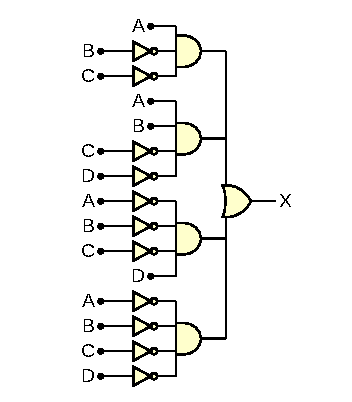
\includegraphics[width=0.5\textwidth]{figures/gateExampleX.pdf}
\caption{\label{fig:gates1} What is the \textit{simplest} expression for the output?}
\end{figure}
\end{enumerate}

\end{document}
